%!TEX root = main.tex

In this chapter, we present our complete solution towards efficient OLAP query processing over property graphs. For comprehensive presentation, we first illustrate the overall solution framework in Section \ref{s:4.1}. Then we present our strategy for materialized view selection, as well as the execution planning for query processing in Section \ref{Materialization Part} and \ref{Future Query Processing Part}, respectively.



%----------------------------------------------------------------------
\section{Solution Framework Overview}
\label{s:4.1}
%----------------------------------------------------------------------

\begin{figure}[H]
	\centering
	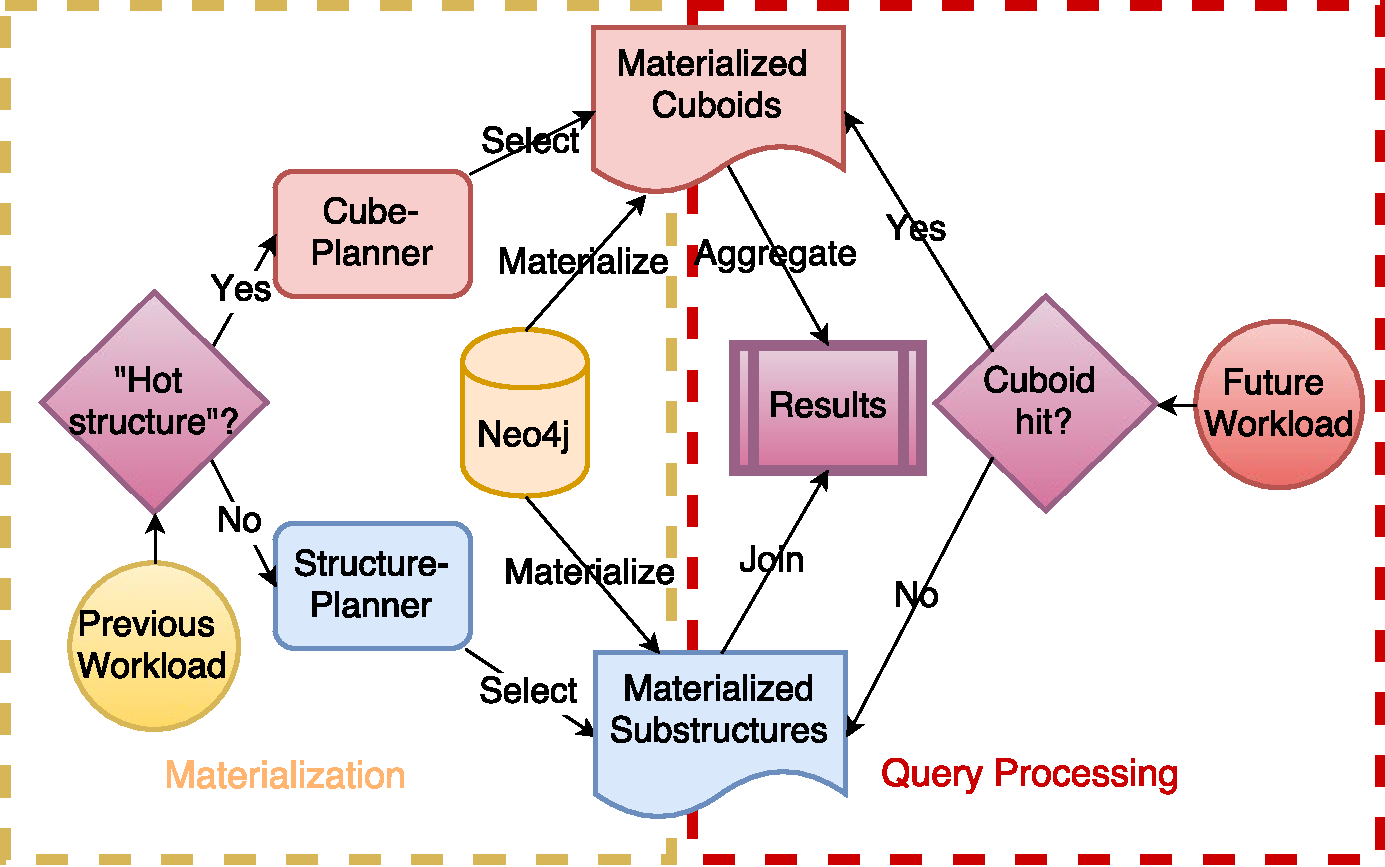
\includegraphics[scale=0.5]{pic/frame.pdf}
	\caption{Solution framework.}
	\label{Solution framework}
\end{figure}

Figure \ref{Solution framework} describes the overall solution framework. Two dashed line rectangles represents the major components of our solution: materialization and query processing. Materialization takes previous workload as input and materializes cuboids and substructures which are beneficial for future workload processing. We adopt a straightforward best effort approach for materialization. Intuitively, we first partition previous queries into ``hot'' queries and ``less hot'' queries based on the frequency count of their structures. Modules CubePlanner and StructurePlanner take ``hot'' queries and ``less hot'' queries as input and produce cuboids and substructures (in form of tables) for materialization respectively. More details are left to Section \ref{Overview of Materialization Part}, where we will explain the intuition of categorization of ``hot'' and ``less hot'' queries, as well as the reason of passing them to different planners.  Query processing component takes incoming queries as input and returns results. Briefly, the workflow of query processing is the following. If a new query happens to contain a ``hot'' structure, we consult cuboid materializations to see if it can be directly answered by aggregation over a cuboid materialization. In this case, cuboid materialization will be used. Otherwise, if the query cannot be directly answered by any materialized cuboid, we consider available materialized substructures by decomposing the query into substructures for join. Note that if required substructure is not materialized, on the fly data fetching from the graph database server is mandatory. %In this case, substructure materializations will be used.

%We will discuss ``Materialization Part'' in Section \ref{Materialization Part} and ``Future Query Processing Part'' in Section \ref{Future Query Processing Part}.




%----------------------------------------------------------------------
\section{Materialized View Selection}
\label{Materialization Part}
%----------------------------------------------------------------------

%We will discuss materialized view selection in this section. We will first give an overview of materialized view selection and then focus on cuboid and substructure selections respectively.
Materialized view selection is a research problem that has attracted significant attention in traditional RDBMS community. However, the fundamental difference between the relational model and the property graph model makes materialization of graph database an interesting topic to explore. This is mainly because \textit{structure} plays an important role in a query over a property graph. One materialized view may affect the benefits of other ones (e.g., when their \textit{structures} overlap). Therefore combinational benefit for a set of materialized views is not a simple sum of benefits for each one of them. As briefly illustrated before, we consider two types of materializations for efficient OLAP query processing: cuboids and substructures. In this section, we first elaborate the essential heuristic of selecting cuboids and substructures. Then we detail the approaches taken for different types of materializations.

%----------------------------------------------------------------------
\subsection{Overview of Materialized View Selection}
\label{Overview of Materialization Part}
%----------------------------------------------------------------------
In Section \ref{Materialization: Cuboid vs Substructures}, we discussed the trade-off between cuboids and substructures. We know that utilization of a cuboid materialization requires future queries to have exactly the same structure as the materialized cuboid. Therefore, it is only reasonable to materialize a cuboid %if TheIt is wise that we materialize a cuboid only
when we are confident that the same structure is likely to be ``hit'' by future queries. Otherwise, it is simply a waste of space to materialize cuboids that would be rarely ``hit''. On the contrary, substructures do not have such strict structural match requirement. A substructure can be used as long as it appears in a future query.

Considering the different features of cuboids and substructures, we take the following strategy for materialized view selection.
%We make our materialization policy based on such different features of cuboids and substructures.
We first perform a frequency count of previous queries. If more than $\omega$ queries shares the same structure, where $\omega$ is a predefined frequency threshold, this structure is considered to be a \emph{hot structure} and would be passed on to the \emph{CubePlanner} module for cuboid selection. Queries that do not have \emph{hot structures} are passed to \emph{StructurePlanner} for the substructure selection. Algorithm \ref{alg:1} describes the overall framework of the materialized view selection process.
%For queries of structure frequency over a threshold $\sigma$, consider these queries have ``hot structure'' and pass them to CubePlanner for cuboid selection. For the rest queries with "less hot structure", pass them to StructurePlanner for substructure selection.

\begin{algorithm}[H]
	\label{alg:1}
	\caption{Materialization Overview}
	\LinesNumbered
	\textbf{System setting:} $\omega$: frequency threshold for hot structures\\
	\KwIn{$Q$: a set of previous queries\\}
	\KwOut{$C$: a set of materialized cuboids\\ $S$: a set of materialized substructures}
	
	$CInput \gets \emptyset$\;
	$SInput \gets \emptyset$\;
	\ForEach{q $\in$ Q}{
		\If{structureFreq(Q, q) $>$ $\omega$}{
			$CInput \gets CInput \cup \{q\} $\;
		}{	
			$SInput \gets SInput \cup \{q\} $\;
		}
	}
	$C$$\leftarrow$\emph{materialize(CubePlanner(CInput))}\;
	$S$$\leftarrow$\emph{materialize(StructurePlanner(SInput))}\;
	\label{alg:PartialMaterialization}
\end{algorithm}
%\clearpage

As shown in Algorithm \ref{alg:1}, function $structureFreq(Q, q)$ returns the frequency count of all query structures in $Q$. After \emph{hot structures} are selected, two functions $CubePlanner$ and $StructurePlanner$  are called to select cuboids and substructures for materialization. Note that we use \emph{materialize()} as a function to denote the materialization of selected cuboids and substructures. To elaborate, consider the following example. Assume we are aware of the six previous queries as shown below. We can group queries by structure and count the structure frequency.


\fbox{\small
	\parbox{\dimexpr\linewidth-2\fboxsep-2\fboxrule\relax}
	{
		\textbf{Previous Workload:} \\
		P1 Badge-User, User-Post:Badge.Name,Post.Score,Post.PostTypeId=2 \\
		P2 User-Comment, Comment-Post: User.UpVotes, Comment.Score, (AVG)Post.Score, Post.PostTypeId=1 \\
		P3 User-Post, Post-Vote: User.UpVotes, Vote.VoteTypeId \\
		P4 User-Post, Post-Tag: (AVG)User.CreationDate\_Year, Tag.TagName \\
		P5 User-Comment, Comment-Post: User.ActiveMonth, Post.CreationDate\_Year=2016 \\
		P6 User-Comment, Comment-Post: User.Age, (AVG)Comment.Score, Post.PostTypeId=2 \\
		\textbf{Future Workload:} \\
		Q1 User-Comment, Comment-Post: User.UpVotes, (AVG)Post.Score, Post.PostTypeId \\
		Q2 User-Comment, Comment-Post: User.Age, Post.PostTypeId \\
		Q3 User-Post, Post-PostHistory: User.UpVotes, PostHistory.PostHistoryTypeId \\
		Q4 Badge-User, User-Post:(AVG)Post.Score,Post.PostTypeId=2
	}
}



%\par
%We count previous queries by structure:

\begin{center}
	\begin{tabular}{ | c | c |}
		\hline
		Structure	&Frequency	\\ \hline
		\textbf{User-Comment, Comment-Post} 	&\textbf{3} \\ \hline
		User-Post, Post-Tag 	&1 \\ \hline
		User-Post, Post-Vote	&1 \\ \hline
	\end{tabular}
	\end {center}
	%\par
	
	Obviously,  \textit{User-Comment, Comment-Post} is a \emph{hot structure}. We materialize cuboids over structure \textit{User-Comment, Comment-Post} by passing previous query P2, P5 and P6 to CubePlanner. CubePlanner will materialize cuboids that benefit processing of future queries Q1 and Q2 (which have \textit{User-Comment, Comment-Post} structure). Then, we pass the three remaining queries of less hot structures,  P1, P3, and P4 to StructurePlanner, which will discover and materialize most useful substructures. In this case StructurePlanner is likely to find \textit{User-Post} as a useful substructure it can be used in joining the result of future queries Q3 and Q4.
	
	
	%----------------------------------------------------------------------
	\subsection{Greedy Selection Framework}
	%----------------------------------------------------------------------
	\label{s:Greedy Selection Framework}
	
	Before diving into the details of the \emph{CubePlanner} and \emph{StructurePlanner} modules, we first illustrate the essential greedy heuristic employed for view selection. %Essentially, we adopt a greedy selection framework in materialized view selection.
	
	In our solution framework, \emph{CubePlanner} and \emph{StructurePlanner} are responsible for materialized view selection (over cuboids and substructures, respectively). They both adopt the same greedy selection framework. In Section \ref{sec:Problem Definition}, we introduced the ``Materialization Selection'' problem, which aims at finding best materializations under a space limit $\sigma$. Materialization selection is a known  NP-complete problem \cite{DBLP:journals/kais/LinK04}. The difficulty lies in that the overall benefit of materialized views is not a simple sum of the individual benefits of each view. A materialized view's marginal benefit may be deducted when another view is selected. For example, the marginal benefit of a substructure over ``\textit{User-Post, Post-Tag}'' will be affected by selecting substructures over ``\textit{User-Post}'' and ``\textit{Post-Tag}''. A straightforward approach to solve the materialization selection problem is to enumerate over all possible combinations of cuboids $C$ and substructures $S$ within the space limit $\sigma$ and find the best combination. But such a brute-force solution is infeasible in practice. In addition, assume that we obtain the optimal $C'$ and $S'$ in some way, it is not guaranteed that the actual total space cost of $C'$ and $S'$ is strictly lower than $\sigma$ as we only made estimations in our calculation. Therefore, we turn to a greedy algorithm which is better than naive approach in terms of efficiency. Besides, it allows materializations to be done one by one while the space limit is strictly respected.
	
	We discuss this greedy selection framework first to give a high-level idea of our selection policy. We use a greedy algorithm for both cuboid and substructure selection, as shown in Algorithm \ref{alg:2}. The idea is to always pick the next candidate with the highest ratio of marginal benefit against the space limit. After a candidate is picked, we re-evaluate the benefit of remaining candidates. Re-evaluation is mandatory as the marginal benefit of a candidate may be reduced as a result of materialization of a selected candidate.
	
	
	\begin{algorithm}[H]
		\label{alg:2}
		\caption{Greedy Selection}
		\LinesNumbered
		\textbf{System setting:} $\sigma$: space limit\\
		\KwIn{$C$: a set of candidates of cuboids or substructures in lattice structure\\ $P$: A set of previous queries}
		\KwOut{$R$: a list of selected candidates to materialize\\ }
		\ForEach{c $\in$ C}{
			c.space $\leftarrow$ space(c)\;
			c.benefit $\leftarrow$ estimateMarginBenefit(c, P, Q)\;
			c.score $\leftarrow$ c.benefit/c.space\;
		}
		
		\While{$Q.totalsize < \sigma$}{
			selected $\leftarrow$ c in C with highest score\;
			R.add(selected)\;
			
			repeat Lines 1-5\;
		}
	\end{algorithm}
	
	%In this algorithm, we use a queue data structure for the output of $Q$. It is because the order of selection is helpful in later computations. %in some cases we may want to keep information of orders of selection.
	%When selection orders are not important we may as well simply use a set to store selected views.
	Lines 1-5 estimate the space cost, the marginal benefit for future workload, as well as the score for each candidate. We call this phase  \textbf{score calculation}. Lines 6-10 keeps picking up candidates with highest score one by one until space limit is hit. Notice that each time a candidate is selected, Line 9 refreshes scores for all candidates by repeating 1-5. We call this phase \textbf{pick-and-update}.
	
	Note that \emph{CubePlanner} and \emph{StructurePlanner} apply this greedy selection framework with different implementations of score calculation and pick-and-update. Users can adjust the behavior of \emph{CubePlanner} and \emph{StructurePlanner} by plugging in their own implementation of the score calculation function that may consider different database features such as execution plans. For the rest of this chapter, we will focus on our implement of  \emph{CubePlanner} and \emph{StructurePlanner} in Neo4j.
	
	%----------------------------------------------------------------------
	\subsection{CubePlanner}
	\label{sec:CubePlanner}
	%----------------------------------------------------------------------
	
	%We will discuss CubePlanner in this subsection.
	\emph{CubePlanner} takes previous queries with \emph{hot structures} as input and returns the selected cuboids for materialization. As mentioned in Section \ref{Materialization: Cuboid vs Substructures}, a cuboid is only useful for queries sharing the exact identical structure. To put it another way, cuboids of different structures do not affect each other at all in terms of benefits for future queries. As a result even though the input queries for \emph{CubePlanner} may have different structures, we can group queries by structure and treat them individually. For each group of input queries, we propose an algorithm named \emph{SingleCubePlanner} to select top-$n$ cuboids. After all groups are finished, we compute the final top-$n$ cuboids by searching across all groups of queries. A good analogy for such a process is to first hold regional competitions and then select national winners from regional winners. Next we will explain \emph{CubePlanner} and \emph{SingleCubePlanner} in detail.
	
	%----------------------------------------------------------------------
	\subsubsection{CubePlanner}
	\label{CubePlanner}
	%----------------------------------------------------------------------
	
	As we mentioned above, \emph{CubePlanner} performs cuboid selection in a holistic manner by  selecting cuboids one-by-one from results of \emph{SingleCubePlanner}. We first explain the workflow of \emph{CubePlanner}, as shown in Algorithm \ref{alg:CubePlanner}. %, then present the \emph{SingleCubePlanners} in details.
	Intuitively, \emph{CubePlanner} first groups $Q$ by structure using the function $group(Q)$. Lines 2-4 perform cuboid selection in each partition using \emph{SingleCubePlanner}. A queue of ordered candidates is generated within each group of queries. Lines 5-8 repeatedly check the current top candidate of each partition to select the best candidate among them. $n$ is a user defined parameter, denoting the most number of cuboids for materialization.  Note that users may choose other ways, such as a space limit, as the bound for cuboid materialization.
	
	\begin{algorithm}%[H]
		\label{alg:CubePlanner}
		\caption{CubePlanner}
		\LinesNumbered
		\textbf{System setting:}
		$n$: maximum number of cuboids to be precomputed\\
		\KwIn{$Q$: a set of previous queries not necessarily with the same structure}
		\KwOut{$C$: a queue of selected cuboids to be precomputed\\ }
		Group$\leftarrow$ group(Q)\;
		\ForEach{group $\in$ Group}{
			group.results $\leftarrow$ SingleCubePlanner(group);
		}
		
		\For{i=1 \emph{\KwTo} n}{
			group' $\leftarrow$ group in Group with highest group.results.top().score\;
			C.offer(group'.Dequeue())\;
		}
		
	\end{algorithm}
	%\clearpage
	
	%Function $group(Q)$ groups $Q$ by structure. $SingleCubePlanner$ will be discussed in Subsection \ref{SingleCubePlanner}.
	
	%Line 1 partitions $Q$ by structure. Each partition consists of previous queries of a same structure, which will be passed to a SingleCubePlanner.
	
	%----------------------------------------------------------------------
	\subsubsection{SingleCubePlanner}
	\label{SingleCubePlanner}
	%----------------------------------------------------------------------
	
	Now we elaborate the \emph{SingleCubePlanner} function. As shown in Algorithm \ref{alg:SingleCubePlanner}, \emph{SingleCubePlanner} follows a greedy selection strategy to generate the top-$n$ cuboids.
	
	\begin{algorithm}%[H]
		\label{alg:SingleCubePlanner}
		\caption{SingleCubePlanner}
		\LinesNumbered
		\textbf{System setting:} $n$: as in ``top-$n$''\\
		\KwIn{$P$: a set of previous queries with a same structure}
		\KwOut{$C$: a queue of selected cuboids to precompute\\ }
		$Lattice \leftarrow buildLattice(Q)$\;
		\ForEach{query $Q$ $\in$ P}{
			$q.time \leftarrow time(q)$\;
		}
		\ForEach{cuboid $\in$ Lattice}{
			$cuboid.space \leftarrow space(cuboid) $\;
			$cuboid.benefit \leftarrow 0$\;
			\ForEach{query $Q$ $\in$ $P$ and q.properties $\subseteq$ cuboid.properties}{
				$cuboid.benefit +=max(0, q.time-aggreTime(cuboid))$\;
			}
			$cuboid.score \leftarrow cuboid.benefit/cuboid.space$\;
		}
		\For{i=1 \emph{\KwTo} n}{
			nextBestCube $\gets$ cuboid in Lattice with highest score\;
			\If{$nextBestCube.score < 0$}{
				break\;
			}
			C.Enqueue(nextBestCube)\;
			\ForEach{cuboid $Q$ $\in$ $Q$ and q.dimension $\subseteq$ nextBestCube.dimension }{
				$q.time \gets min(q.time, aggreTime(nextBestCube)) $\;
			}
			Repeat 5-12\;
		}
		
	\end{algorithm}
	%\clearpage
	
	
	The algorithm starts with building a lattice over all combinations of dimensions of all attributes that appeared in previous query set $P$, using a classic lattice construction algorithm described in \cite{DBLP:journals/ipl/NourineR99}. Lines 2-4 initialize the best-so-far processing time for each previous query with its estimated naive database processing time. Lines 5-12 perform score calculation following the greedy selection framework presented in Algorithm \ref{alg:1}. For each cuboid, we estimate its space (line 6). Lines 8-10 calculate the marginal benefit by iterating over previous queries that can be answered by scanning current cuboid. If the estimated scanning time is less than a previous query's current best-so-far processing time, we add the difference of two times to the cuboid's total marginal benefit (Line 9). Lines 13-23 perform the pick-and-update, where lines 15-17 terminate the selection process when there is no more extra marginal benefit, and lines 19-22 update the best-so-far processing time for previous queries as a result of the current round of selection.
	
	Now we explain the implementation details of the time estimation function employed in Algorithm \ref{alg:SingleCubePlanner}.
	%Implementation of functions are listed as follows. Notice that users can implement these functions in their own ways based on their database systems.
	Function \textbf{$time(query)$} estimates the time of na\"ive  processing of a query in a graph database. Implementation of $time(query)$ is database specific as physical storage and execution plans vary among different databases (i.e., not using materialized views). Since Neo4j provides APIs to show the execution plan as well as the estimated intermediate result size, we directly use the total size of intermediate results as an estimation of the time cost. For example, Figure \ref{fig:4:2} is an execution plan provided by Neo4j for query \textit{User-Badge, User-Post, Post-Tag: Tag.TagName}. We can see that the number of estimated rows of intermediate results are provided. We use the sum of estimated rows to estimate the total processing time cost.
	
	%explain match (:Badge)-[]-(u:User)-[]-(p:Post)-[]-(t:Tag) return count(t.TagName)
	
	\begin {figure}[H]
	\centering
	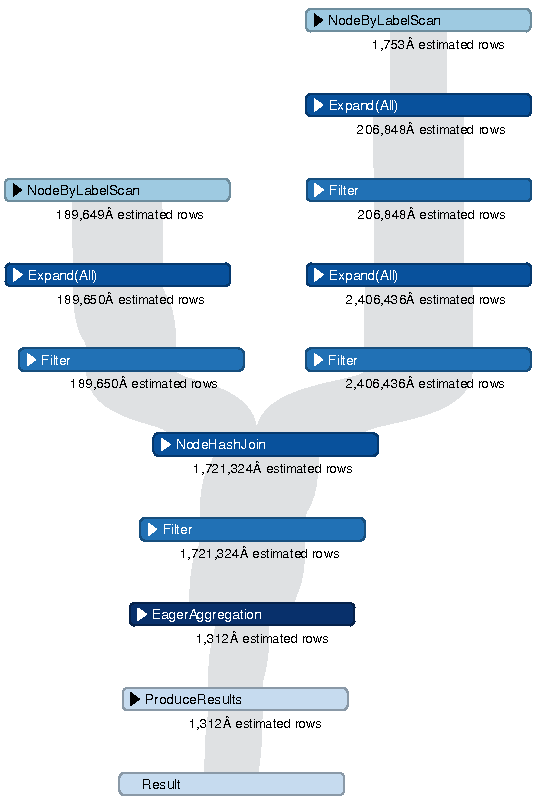
\includegraphics[scale=1.3]{pic/eplan.pdf}
	\caption{Neo4j's execution plan for query \textit{User-Badge, User-Post, Post-Tag: Tag.TagName}.}
	\label{fig:4:2}
\end{figure}

For graph databases that do not provide an API to access execution plans and estimated intermediate result sizes, users can construct different estimation functions following the same intuition, which usually depends on specific database implementations. There are many studies on cost estimation for database operations (e.g., join operation). Users may consider joining (expanding) order \cite{DBLP:conf/pods/Chaudhuri98} and estimation of intermediate result sizes  \cite{DBLP:conf/edbt/SwamiS94} as two important factors.

Function \textbf{$aggreTime(cuboid)$} estimates the time cost for scanning a materialized cuboid. Given a cuboid $c$, we estimate the space cost of $c$ as follows:


\begin{displaymath}
spacePerRow = 
\displaystyle{\sum_{p\in c.properties}sizeOf(p)}
\end{displaymath}

\noindent Thus,
\begin{displaymath}
SpaceCost(c) = spacePerRow \times numberOfRows(c)
\end{displaymath}
Note that \textit{sizeOf(property type)} refers to the standard size of data types. For example, the integer type in ``C++'' is 2 byte. \textit{numberOfRows(c)} refers to the number of rows in $c$. A rough estimation is the size of the Cartesian product of all queried properties:

\begin{displaymath}
numberOfRows(c) = \displaystyle{\prod_{p\in c.properties}|p|}
\end{displaymath}


%----------------------------------------------------------------------
\subsection{Structure Planner}
\label{Structure Planner}
%----------------------------------------------------------------------
As mentioned above, \emph{StructurePlanner} also adopts the same greedy selection strategy described in Algorithm \ref{alg:1}. We detail the process of \emph{StructurePlanner} in Algorithm \ref{alg:StructurePlanner}. First, we build a lattice over all substructures contained in previous queries $P$, using the classic lattice construction algorithm (similar to the lattice construction algorithms adopted in \emph{CubePlanner}). Figure \ref{fig:4:3} shows a substructure lattice originating from the root node \textit{Badge-User, User-Post, Post-Tag}. Starting from a union of structures of previous queries as the root node, a lattice can be constructed recursively by populating descendants from parent nodes through edge removals.

\begin {figure}[h]
\centering
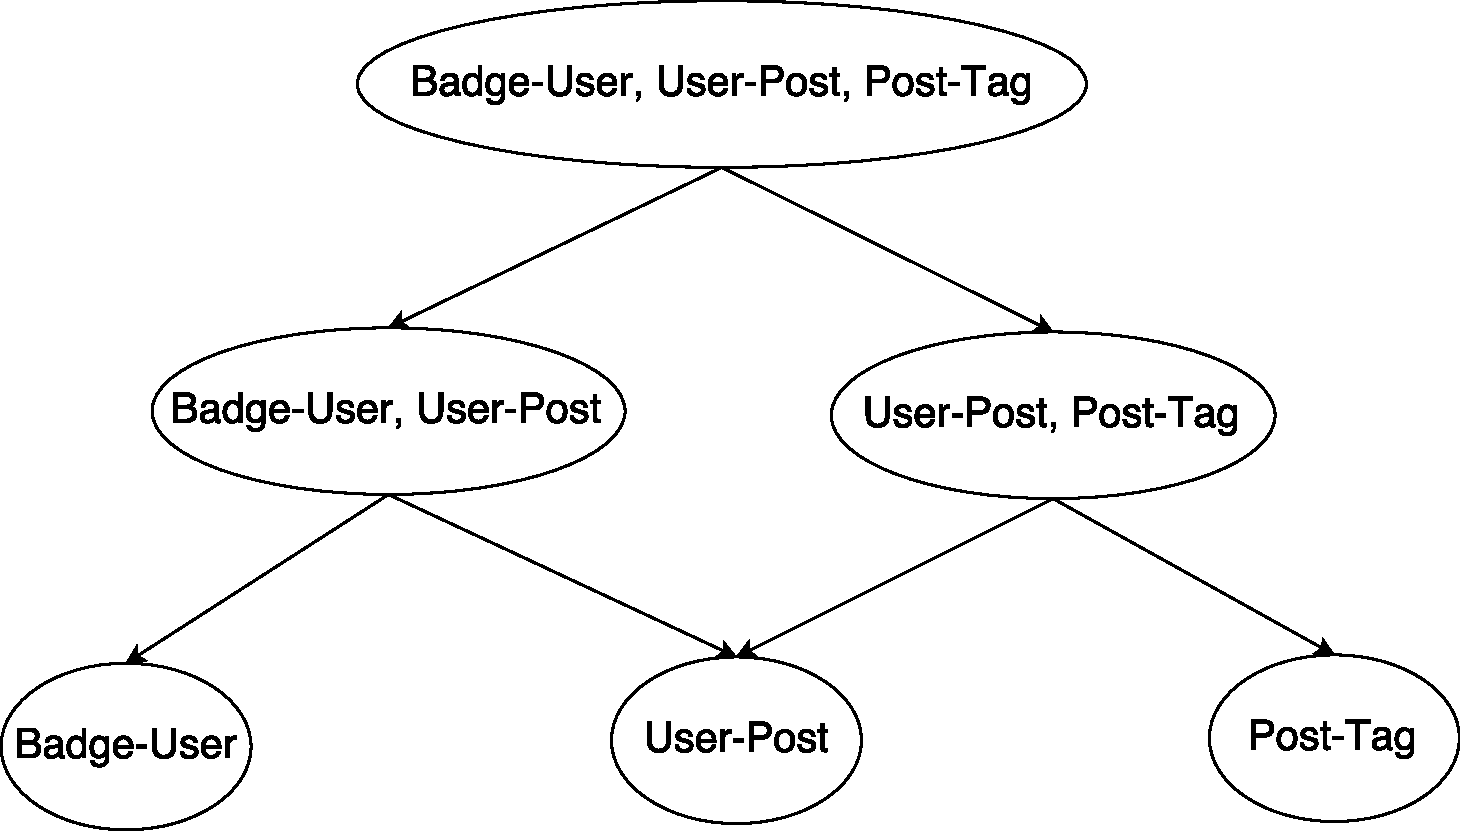
\includegraphics[scale=0.45]{pic/slattice.pdf}
\caption{A substructure lattice with \textit{Badge-User, User-Post, Post-Tag} as its root node.}
\label{fig:4:3}
\end{figure}


Then, we initialize the covered substructures for each previous query as an empty set (lines 2-4). For a previous query, $coveredSubstructure$ keeps the information on what substructures have been selected so far. %, which are useful for processing this query.
It is updated every time a new substructure is selected. Lines 5-12 perform score calculation. For each substructure, Line 6 estimates its space. Lines 8-10 iterate over all ``favored'' previous queries (favored by current substructure) and add on the marginal benefit (if any). Here marginal benefit refers to the time saved after adding current substructure to selected substructures (Line 9). Lines 13-23 perform the pick-and-update, and lines 19-22 update the covered substructures for previous queries as a result of current round of selection. Such iteration will be terminated when space limit is exceeded (line 13) or when there is no more marginal benefit (line 15).

\begin{algorithm}%[H]
\label{alg:StructurePlanner}
\caption{StructurePlanner}
\LinesNumbered
\textbf{System setting:} $\sigma$: space limit for materialized views\\
\KwIn{$Q$: a set of previous queries}
\KwOut{$S$: an queue of selected substructures to precompute\\ }
$Lattice \leftarrow buildSubstuctureLattice(Q)$\;
\ForEach{q $\in$ Q}{
	$q.coveredSubstructres\leftarrow \emptyset $\;
}
\ForEach{substructure $\in$ Lattice}{
	$substructure.space \leftarrow space(substructure) $\;
	$substructure.benefit \leftarrow 0$\;
	\ForEach{q $\in$ $Q$ and q.structure $\subseteq$ substructure.structure}{
		$cuboid.benefit +=max(0, benefit(q, substructure, q.coveredSubstructres))$\;
	}
	$substructure.score \leftarrow substructure.benefit/substructure.space$\;
}
\While{$System.memoryUsage < \sigma$}{
	nextBestSubstructre $\gets$ substructure in Lattice with highest substructure.score\;
	\If{$nextBestSubstructre.score < 0$}{
		break\;
	}
	S.offer(nextBestSubstructre)\;
	\ForEach{q $\in$ $Q$ and q.structure $\subseteq$ nextBestSubstructre.structure }{
		$q.coveredSubstructres \gets q.coveredSubstructres \cup \{nextBestSubstructre \} $\;
	}
	repeat 5-12\;
}
\end{algorithm}
%\clearpage

We now explain the detailed implementation of the estimation functions employed in Algorithm \ref{alg:StructurePlanner}. Note that these are specific to our implementation in Neo4j and may differ in the case of other systems. Function \textit{space(substructure)} returns the estimated space cost of a substructure materialization. We use Neo4j's execution plan API to get an estimated result size of a substructure. Function \textit{benefit(q, substructure, q.coveredSubstructres)} evaluates the marginal benefit of materializing a substructure for $Q$. We know that execution plan and estimated intermediate result size are provided by Neo4j's API. But when substructure materialization is used, the actual execution plan (intermediate result) may be different than the na\"ive processing plan. As a result, estimating the marginal benefit of a substructure is tricky. We estimate the marginal benefit of a substructure using
\begin{displaymath}
time(q.coveredSubstructres \cup substructure) - time(q.coveredSubstructres),
\end{displaymath}
\noindent which captures the overall improvement of adding $substructure$ to $coveredSubstructres$ as materializations.


%----------------------------------------------------------------------
\subsection{ID and Property Selection}
%----------------------------------------------------------------------

Given a substructure picked by the \emph{StructurePlanner}, we need to decide  which IDs and properties need to be stored. Keeping all IDs and attributes makes a substructure materialization more informative but increases the space cost. %We are faced with a trade-off between space cost and usage potential.
Thus, the selection of IDs and properties is an important issue. We  use substructure \textit{User-Post, Post-Tag} as an example and discuss different ID and property selection policies.

For IDs, we consider the following two policies.

\begin{itemize}
\item Policy \#1 keeps IDs of all nodes and edges. For \textit{User-Post, Post-Tag}, if we keep IDs of all nodes and edges, then we can perform join operation with \textit{Badge-User, User-Post}. We call such join an ``overlap join'' as the two substructures have an overlap part which is \textit{User-Post}. Note that we can join the two substructures only when IDs of nodes (User and Post), and edge (edge between User and Post) are stored in both substructures.

\item Policy \#2 only keeps IDs of ``border nodes'' which are on the border of the substructure's \textit{structure}. Figure \ref{border node} highlights ``border nodes'' of structure \textit{User-Post, Post-Tag}. In this example we only save IDs of User and Tag. We do not keep IDs of Post as node Post is not located on the border of the \textit{structure}. This saves space compared with Policy \#1, however Policy \#2 only enables joins on border nodes. For example we may join \textit{User-Post, Post-Tag} with \textit{User-Badge} on their common border node User. But ``overlap join'' with other substructures is not enabled because IDs of ``inner nodes'' are not stored. We cannot join \textit{User-Post, Post-Tag} with \textit{Badge-User, User-Post} as Post is an ``inner node'' and IDs of Post is not stored. 

\begin{figure}[h]
	\centering
	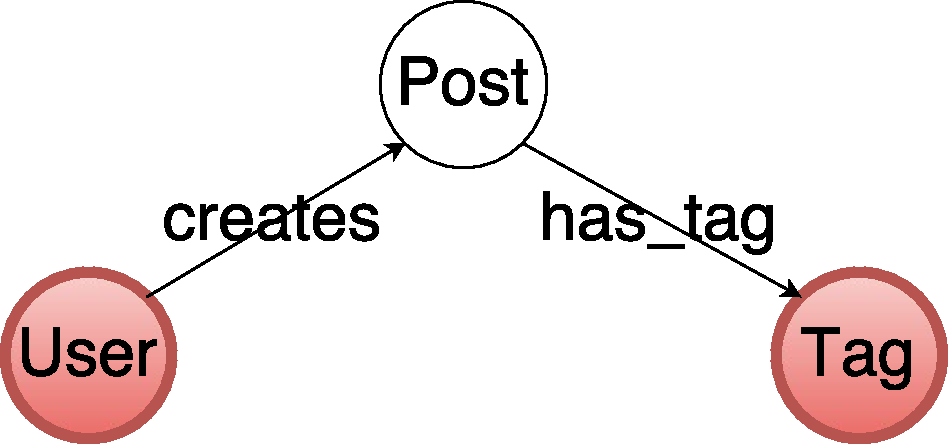
\includegraphics[scale=0.35]{pic/bordernode.pdf}
	\caption{``Border nodes'' of structure \textit{User-Post, Post-Tag}.}
	\label{border node}
\end{figure}
\end{itemize}


We use Policy \#1 in our implementation. However if keeping IDs of inner nodes and edges overwhelmingly increases result length, it's wise to choose Policy \#2 as space cost becomes too high.

For properties, we consider the following two policies.

\begin{itemize}
\item Policy \#1 keeps all properties.
\item Policy \#2 only keeps properties that were queried in previous workloads.
\end{itemize}

Our suggestion is to consider the proportion of properties which were queried in previous workload over all properties in the data schema. For example, in our experiment only a small proportion of properties were queried. We choose Policy \#2 as it is a waste of space to keep all properties.

%\intodo{Please add a short section discussing how to update the materialized views. For example, along the execution of more and more queries, there could be change of ``hot structures''. How we update the materialized views, or possible solutions to address this problem.}

%----------------------------------------------------------------------
\subsection{Update on Materialized Views}
%----------------------------------------------------------------------
The solution we have discussed so far is applicable for static scenarios (with fixed previous workload). We now expand our solution to dynamic scenarios: as queries are executed, there could be change of ``hot structures'' and ``properties of interest''. Thus updates on materialized views are necessary. Remember that we have a memory budget, therefore in some cases obsolete materialized views need to be swapped out for new ones. To achieve this, we maintain a sliding window over previous queries. After executing a certain number of queries, we perform materialized view selection over only ``recent queries'' which are in the sliding window. Old views that need to be swapped out are eliminated by simply releasing their memory. For newly selected views we materialize them. For old views that do not need to be swapped out, we do nothing as they are already materialized in memory. In this way periodical update on materialized views can be realized.


%----------------------------------------------------------------------
\section{Query Processing}
\label{Future Query Processing Part}
%----------------------------------------------------------------------
Query processing aims at processing incoming queries efficiently using materialized substructures and cuboids. When a query $q$ arrives, we first consult materialized cuboids. If $q$ can be answered with an aggregation over any materialized cuboid, we select the cuboid with the minimum space and directly scan over it to produce result of $q$. If $q$ cannot be answered by any cuboid, we decompose $q$ and use substructures as much as possible to compute the result of $q$.

\begin{algorithm}[H]
\label{alg:Query Processing}
\caption{Query Processing}
\LinesNumbered
\textbf{System:} $C$: a set of materialized cuboids\\ $S$: a set of materialized substructures\\
\KwIn{$q$: a query\\}
\KwOut{$r$: result of $q$}

$minspace\leftarrow \infty $\;
mincuboid \leftarrow NULL\;
\ForEach{$cuboid \in C$}{
	\If{cuboid.structure = q.structure and q.dimension $\subseteq$ cuboid.dimension}{
		\If{$cuboid.space<minspace$}{
			minspace \leftarrow cuboid.space\;
			mincuboid \leftarrow cuboid\;
		}
	}
	
	\eIf{$mincuboid \not= NULL$}{
		$r \leftarrow aggregate(mincuboid, q)$\;
	}{
		$r \leftarrow Decompose\_Join(q)$\;
	}
}
\end{algorithm}
%\clearpage

Algorithm \ref{alg:Query Processing} describes the generic work flow of query processing. Given an incoming query $q$,
we first look up materialized cuboids and find if any cuboid can be used to answer $q$ (lines 4-9). Note that $cuboid.space$ in line 5 was computed in line 9 in Algorithm \ref{alg:SingleCubePlanner}. Then, we check if $q$ can be answered by cuboid materialization. If so, we perform aggregation operation over the cuboid (line 11). Otherwise, we need to decompose $q$ into substructures and compose the result (line 13). Function $aggregate(mincuboid, q)$ is the classic aggregation operation. We will discuss how function $Decompose\_Join(q)$ is implemented at the end of this section.

%----------------------------------------------------------------------
\subsection{Substructure Selection}
\label{Substructure Selection}
%----------------------------------------------------------------------

Before discussion on $Decompose\_Join(q)$, we need to first solve a ``Substructure Selection'' problem. In order to decompose a query $q$, we need to consider which materialized substructures we need to use. We need to make decision when candidate substructures in $S$ overlap. For example suppose $q$ has structure \textit{Badge-User, User-Post, Post-Tag}.

And S consists of substructures

(1) Badge-User

(2) Badge-User, User-Post

(3) User-Post, Post-Tag

(4) Post-Tag

(5) User-Post.

We can get structure of $q$ by joining structures of (1) and (3). Thus (1) and (3) seem to be a possible combination for substructure selection in this case. Actually we may have at least three possible substructure selections: (1) and (3); (2) and (4);
(1), (4) and (5). The key question is which selection will result in fastest processing time on $q$? Here are some intuitions to solve this tricky question. First, when we select substructures one by one, we do not select a substructure when it is covered by selected substructures. For example we will not consider (1) if (2) has been selected as (1) is covered by (2). Second, we prefer to minimize total size of selected substructures as we need to at least access each selected view once. We prefer less memory access. Third, we prefer smaller number of selected substructures as intuitively this causes less times of joins.

We propose a greedy algorithm for substructure selection based on user defined heuristics. Users may define heuristic functions based on intuitions (like the three intuitions mentioned above). The idea of the greedy algorithm is to always pick up next substructure with highest score of user defined heuristic function $h(s)$, which returns heuristic score for a substructure $s$. Some example heuristics are \#edges of substructure, score calculated in StructurePlanner (Line 11 in Algorithm \ref{alg:StructurePlanner}), table size etc.

\begin{algorithm}[H]
\caption{SelectSubstrucre}
\label{alg:SelectSubstrucre}
\LinesNumbered
\textbf{System:} $S$: a collection of materialized substructures\\ $h(s)$: user defined function. It returns the heuristic score of a substructure $s$.\\
\KwIn{$q$: a future query\\}
\KwOut{$V$ : selected views for future joining\\ $uncoveredStruc$: structure not covered by selected views\\$uncoveredProp$: properties not covered by selected views\\}
uncoveredStruc \leftarrow q.structure\;
uncoveredProp\leftarrow q.properties\;
$coveredStruc\leftarrow \emptyset$\;
$V\leftarrow\emptyset $\;
\ForEach{$s \in S$ ordered by h(s)}{
	\If{s $\subseteq$ uncoveredStruc and s $\not\subseteq$ coveredStruc}{
		$V \leftarrow V \cup \{s\}$\;
		$coverdStruc \leftarrow coveredStruc \cup s.structure$\;
		uncoveredStruc \leftarrow uncoveredStruc - s.structure\;
		uncoveredProp \leftarrow uncoveredProp -s.properties\;
	}
}
\end{algorithm}
%\clearpage

Lines 1-2 initialize $uncoveredStruc$ and $uncoveredProp$, which keeps track of structures and properties which have not been covered by selected substructures. Such uncovered structures and properties will need to be fetched from the database. Line 3 initializes $coveredStruc$, which keeps union of selected substructures. Line 5 starts iteration over substructures ordered by user-defined heuristics $h(s)$. Line 6 assures that a candidate substructure that is totally covered by selected substructures will be disqualified. In the above example, suppose we have already selected (2), there is no need to select (1) since (1) is totally covered by (2).

%----------------------------------------------------------------------
\subsection{Decomposition and Join}
\label{Query Decomposition}
%----------------------------------------------------------------------
In this section, we  discuss how to implement function $Decompose\_Join(q)$ (as in Algorithm FutureQueryProcessing in subsection \ref{Future Query Processing Part}). Besides $Decompose\_Join(q)$, we shall discuss two other variations of implementation: $Decompose\_Join^{*}$ and $Decompose\_Join^{+}$.

%----------------------------------------------------------------------
\subsubsection{\#1 $Decompose\_Join$}
%----------------------------------------------------------------------
Given a query $q$, we use the previously discussed algorithm ``SelectSubstrucre'' to select a set of substructure materializations $V$. However, substructures in $V$ may not completely cover the structure of $V$. If there is any remaining structure ($uncoveredStruc$) and properties ($uncoveredProp$) that $V$ does not cover, we need to retrieve them from the database. We call such remaining structures and properties fetched from the database ``complementary  components''. After all these components (both materializations and ``complementary  components'') are finally ready, we join and aggregate them to produce final results.

\begin{algorithm}[H]
\caption{Decompose\_Join}
\LinesNumbered
\textbf{System:} $S$: a collection of materialized substructures\\
\KwIn{$q$: a future query\\}
\KwOut{$r$: result of $q$}
$\Sigma \gets \emptyset $\;
$V, uncoveredStruc, uncoveredProp \gets SelectSubstrucre(q) $\;
$\Sigma \gets \Sigma \cup V $\;
$Splits\leftarrowsplit(uncoveredStruc, uncoveredProp)$\;
\ForEach{s: Splits}{
	$\Sigma \gets \Sigma \cup \{retrieve(s)\} $\;
}
$r \leftarrow join\_aggregate(\Sigma, q)$\;
\end{algorithm}

Line 1 initializes $\Sigma$, which maintains a set of all components (materializations and ``complementary  components'') that are needed. Line 2 selects substructures using SelectSubstructure algorithm. $uncoveredStruc$ and $uncoveredProp$ refer to structures and properties which are not covered by selected substructures. They are ``complementary components'' and will be retrieved from database servers. Line 4 splits $uncoveredStruc$ and $uncoveredProp$ into connected components. We retrieve each connected component from the database server. Note that splitting is necessary since $uncoveredStruc$ may not be exactly one connected component. Line 8 joins and aggregates all materials together to produce results.

Function \textit{split(uncoveredStruc, uncoveredProp)} is implemented by a classic connected components detection algorithm. It splits $uncoveredStruc$ and $uncoveredProp$ into connected components (structures). We want to retrieve each connected structure separately from the database because otherwise it may result in unnecessarily large results of Cartesian products of several disconnected structures. Function \textit{$materialize(s)$} retrieve ``complementary components'' $s$ from the database server. Function \textit{join($\Sigma$, q)} join tables of $\Sigma$ together and aggregate over properties based on $q$. Joins over multiple tables is a well-studied topic. Joining order and join technique (hash join etc.) are two important aspects of this topic. In our implementation we use hash join and our joining order policy is to keep joining two tables which have minimum sum of table sizes and have common column(s). That is, we tend to select two smaller tables to join.

%----------------------------------------------------------------------
\subsubsection{\#2 $Decompose\_Join^{*}$}
%----------------------------------------------------------------------
$Decompose\_Join$ retrieve ``complementary components'' from the database in a naive manner. We adopt the idea of Semi-Join \cite{DBLP:journals/dr/Ozsoyoglu99} and propose another way of implementation: $Decompose\_Join^{*}$. Semi-join takes advantage of ``selection effect'' of natural joins. In $Decompose\_Join^{*}$, we first perform joins over substructures of $V$ even before fetching ``complementary components'' from the database. Line 3 performs $join(V)$ before $retrieve$ in Line 7. We call this phase ``first round of joins''.  Note that substructures in $V$ may reside in multiple connected components. Thus $V^{*}$ may consist of multiple intermediate tables. The purpose for first round of joins is that it provides ``candidate'' node and edge IDs for future joins (thanks to `selection effect'' of natural joins). When fetching ``complementary components'' from the database server, we inform database server such candidate node and edge IDs so that search space for ``complementary components'' is narrowed down ($retrieve^{*}(s, V^{*})$ in Line 7). We name this approach $Decompose\_Join^{*}$.

\begin{algorithm}[H]
\caption{$Decompose\_Join^{*}$}
\LinesNumbered
\textbf{System:} $S$: a collection of materialized substructures\\
\KwIn{$q$: a future query\\}
\KwOut{$r$: result of $q$}
$\Sigma \gets \emptyset $\;
$V, uncoveredStruc, uncoveredProp \gets SelectSubstrucre(q) $\;
$V^{*}\leftarrowjoin(V)$\;
$\Sigma \gets \Sigma \cup V $\;
$Splits\leftarrowsplit(uncoveredStruc, uncoveredProp)$\;
\ForEach{s: Splits}{
	$\Sigma \gets \Sigma \cup \{retrieve^{*}(s, V^{*})\} $\;
}
$r \leftarrow join\_aggregate(\Sigma, q)$\;
\end{algorithm}
%\clearpage


We explain implementation of function $retrieve^{*}(s, V^{*})$. It fetches results from the database by passing candidate IDs information (from join result $V^{*}$). Syntax to achieve this varies by database. In SQL and Cypher we may pass candidate IDs using a ``WHERE'' statement. Besides Neo4j driver supports passing lists of integers as arguments in a query.


We compare $Decompose\_Join^{*}$ vs.  $Decompose\_Join$ and summarize following pros and cons of $Decompose\_Join^{*}$. $Decompose\_Join^{*}$ helps accelerate retrieval process from back end databases in two aspects. First, since screened out candidate IDs are provided, database back end only needs to iterate through a portion of nodes and edges. This saves database processing time. Second, candidate IDs have a ``selection'' effect thus size of retrieval results is deducted. Thus time caused by result transmission will be reduced. The disadvantages are twofold. First, $Decompose\_Join^{*}$ has to transmit IDs. Second,  $Decompose\_Join^{*}$ performs two rounds of join; first on $V$ before ``complementary components'' are ready,  followed by second round of joins. In terms of optimization on join orders, $Decompose\_Join$ is better because its join order is decided over all the tables, whereas in $Decompose\_Join^{*}$ tables are separated by two rounds of joins, which narrows down the scope of all possible join orders.

------------------
\subsubsection{\#3 $Decompose\_Join^{+}$}
%----------------------------------------------------------------------
We mentioned two advantages of $retrieve^{*}(s, V^{*})$. However a disadvantage of $retrieve^{*}(s, V^{*})$ is an overhead of transmission of candidate IDs. We propose a decisive way to evaluate the trade-off between overhead and benefits of $retrieve^{*}(s, V^{*})$ and choose between $retrieve^{*}(s, V^{*})$ and $retrieve(s)$. $Decompose\_Join^{+}$ is derived from $Decompose\_Join^{*}$. The trick is to revise Line 7 by using $decide(s,V^{*})$ to choose the better way between $retrieve^{*}(s, V^{*})$ and $retrieve(s)$.

\begin{algorithm}[H]
\caption{$Decompose\_Join^{+}$}
\LinesNumbered
\textbf{System:} $S$: a collection of materialized substructures\\
\KwIn{$q$: a future query\\}
\KwOut{$r$: result of $q$}
$\Sigma \gets \emptyset $\;
$V, uncoveredStruc, uncoveredProp \gets SelectSubstrucre(q) $\;
$V^{*}\leftarrowjoin(V)$\;
$\Sigma \gets \Sigma \cup V $\;
Splits\leftarrowsplit(uncoveredStruc, uncoveredProp)\;
\ForEach{s: Splits}{
	\eIf{decide(s,$V^{*}$)}{
		$\Sigma \gets \Sigma \cup \{retrieve^{*}(s, V^{*})\} $\;
	}{
		$\Sigma \gets \Sigma \cup \{retrieve(s)\} $\;
	}
}
$r \leftarrow join\_aggregate(\Sigma, q)$\;
\end{algorithm}
%\clearpage

Implementation of function $decide(s,V^{*})$ is detailed as follows. We first estimate result sizes of the two retrieval methods: $retrieve^{*}(s, V^{*}).estSize$ and $retrieve(s).estSize$. $retrieve(s).estSize$ can be returned by $space(substructure)$ in Algorithm \ref{alg:StructurePlanner}. The tricky one is $retrieve^{*}(s, V^{*}).estSize$, whcih we estimate as follows:
\begin{enumerate}
\item  Randomly sample a small number of candidate IDs.

\item  Execute $retrieve^{*}$ but pass only sampled candidate IDs in (1). We call this a ``trial query''. We want to use the ``trial query'' to estimate result length of actual $retrieve^{*}(s, V^{*})$. Since we only pass a small number of IDs, time cost of ``trial query'' is acceptably small.

\item  Calculate $retrieve^{*}(s, V^{*}).estSize$ proportionally using the result of ``trial query''.
\end{enumerate}
\par
We compare $retrieve^{*}$'s benefit in result size reduction against its cost in passing candidate IDs by evaluating $(retrieve(s).estSize - retrieve^{*}(s, V^{*}).estSize) / sizeOf(candidateIDs)$ and compare the ratio with a threshold $\gamma$ and make a decision. $\gamma$ is important as it directly affects decision making. We suggest running some prior tests in order to adjust $\gamma$ to a proper value. The prior tests are conducted by executing some sample queries by both $Decompose\_Join$ and $Decompose\_Join^{*}$. In each test, the value of $(retrieve(s).estSize - retrieve^{*}(s, V^{*}).estSize) / sizeOf(candidateIDs)$, together with correct decision between $Decompose\_Join$ and $Decompose\_Join^{*}$ (the one with less processing time) are recorded. We view it as a binary classification problem and  it can be easily solved by linear regression.   

We compare  $Decompose\_Join^{+}$ vs $Decompose\_Join^{*}$: We see that $Decompose\_Join^{+}$ performs two rounds of joins like $Decompose\_Join^{*}$. The major difference is that $Decompose\_Join^{+}$ plays ``trial query''. The principle behind ``trial query'' is to pay an acceptable price to make a wise decision on ``complementary components'' retrieval. Our experiments show that a good decision making on ``complementary components'' retrieval saves much more time than the time cost of ``trial queries'', results and discussion of which will be presented in next chapter.




%----------------------------------------------------------------------
